\begin{figure}[h]
  \centering
  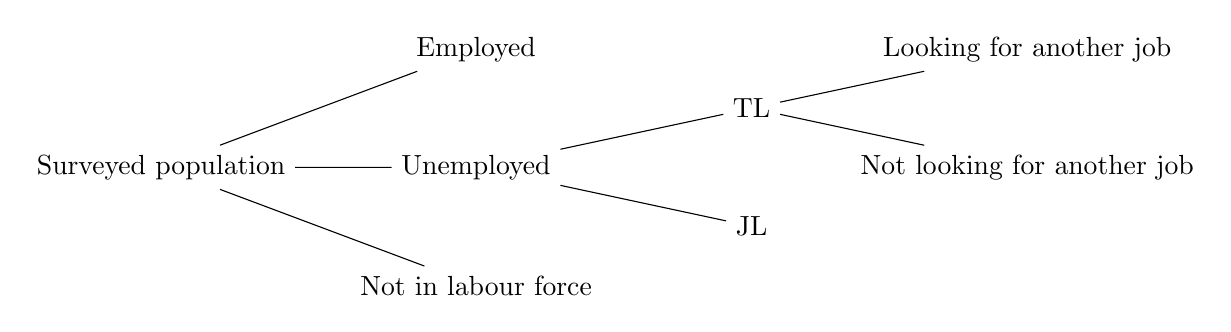
\begin{tikzpicture}[grow=right]
    \tikzset{level 1/.style={level distance = 4cm}}
    \tikzset{level 2/.style={level distance = 3.5cm}}
    \tikzset{level 3+/.style={level distance = 3cm}}
    \node{Surveyed population}
      child{node{Not in labour force}}
      child{node{Unemployed}
        child{node{JL}}
        child{node{TL}
          child{node{Not looking for another job}}
          child{node{Looking for another job}}
        }
      }
      child{node{Employed}}
    ;
  \end{tikzpicture}
  \caption{Tree structure of labour market status in CPS.}
  \subcaption*{TL = Temporary layoff, JL = Job-less unemployment (unemployment for any other reasons than temporary layoff). Definitions for the classifications are provided in the body text.}
  \label{cps_tree}
\end{figure}